\chapter{Identification of Tools and Techniques}
\label{ch:tools}

\section{Development Tools}
\label{sec:devtools}
The system uses tools chosen for scalability, compatibility, and their support for machine learning, data analysis and pipeline integration.

\textbf{Python 3.11} is the primary programming language, chosen for its simplicity, cross-platform support and extensive ecosystem of machine learning and data processing libraries. All package versions are pinned so that saved model artifacts load exactly as trained.

\textbf{Scikit-learn}~\cite{pedregosa2011scikit} implements Random Forest, Decision Tree and Support Vector Machine for build failure prediction, along with Isolation Forest, TF-IDF and k-means for anomaly detection and log clustering, and the evaluation metrics.

\textbf{LightGBM}~\cite{ke2017lightgbm} and \textbf{XGBoost}~\cite{chen2016xgboost} provide gradient-boosted trees. LightGBM also provides the learning-to-rank objective used by the final model.

\textbf{Pandas, NumPy and PyArrow} are used for data preprocessing, cleaning, feature extraction, numerical computation and efficient storage of the 3.56 million-row Travis~CI data.

\textbf{SHAP}~\cite{lundberg2017unified} explains individual predictions by attributing each prediction to its input features.

\textbf{Visual Studio Code} is the main development environment, and \textbf{pytest} runs the automated test suite.

Deep learning frameworks (TensorFlow, PyTorch) were planned for possible future use. They were not needed: tree ensembles performed well, are faster to train, and are easier to explain.

\section{CI/CD and Integration Tools}
\label{sec:citools}
\textbf{GitHub Actions} is a cloud-based CI/CD platform tightly coupled with GitHub repositories. In this project it plays three roles:
\begin{itemize}
\item \textbf{Data source:} workflow runs, commits and job timings of 60 public repositories were collected through its API.
\item \textbf{Live input:} the deployed system receives signed \texttt{workflow\_run} and \texttt{workflow\_job} webhook events and scores each run when it is requested.
\item \textbf{CI for this project:} every pull request runs the backend tests and a production build of the dashboard.
\end{itemize}

\textbf{Travis~CI}, through the TravisTorrent dataset~\cite{beller2017travistorrent}, provides the main development data: 3.56 million job records from 947 projects.

\textbf{Jenkins} is one of the most widely used open-source CI/CD automation servers. The system provides a Jenkins notification endpoint protected by a shared secret, so Jenkins builds can be recorded and scored as well.

\textbf{GitHub} hosts the project's code and is used for version control, pull requests and releases. Commit activity on GitHub, such as code churn, files changed and commit timing, also provides important model features.

\section{Visualization and Deployment Tools}
\label{sec:viztools}
The design originally proposed Grafana and Kibana for visualization. Instead, a purpose-built \textbf{React} dashboard was implemented with \textbf{Vite}, \textbf{Tailwind CSS} and \textbf{Recharts}. It shows exactly the project's outputs: failure risk, alerts, trends, explanations, bottlenecks and model evidence. It uses animated, colorblind-checked charts, and every chart has a legend or labels. The backend is a \textbf{FastAPI} service with a \textbf{SQLite} database (via SQLAlchemy). \textbf{ReportLab} generates per-build PDF reports.

\textbf{Docker} packages the service. A read-only public demonstration runs as a single container on \textbf{Render}, serving the dashboard and the API from one address.

\section{Techniques Used}
\label{sec:techniques}

\minorhead{Random Forest}
Random Forest~\cite{breiman2001random} is an ensemble of decision trees trained on random subsets of data and features. It is robust against overfitting and handles mixed, complex features well. In this project it is the main baseline: \tierC, a Random Forest with repository history, is the model that \tierE\ is compared against.

\minorhead{Decision Tree}
A Decision Tree~\cite{quinlan1986induction} classifies data with a hierarchy of decision rules derived from the features. It is interpretable, which helps explain what drives pipeline failures. It was trained and compared as planned.

\minorhead{Support Vector Machine (SVM)}
SVM~\cite{cortes1995support} finds the boundary that best separates classes in a high-dimensional feature space. It was evaluated against Random Forest and Decision Tree using accuracy, precision, recall and F1-score.

\minorhead{Gradient Boosting and Learning to Rank}
Gradient boosting (XGBoost~\cite{chen2016xgboost}, LightGBM~\cite{ke2017lightgbm}) builds trees sequentially, each correcting the errors of the previous ones. A team's real question is ``which of \emph{our} builds are riskiest?'', so the final model also uses a \emph{learning-to-rank} objective, XE-NDCG~\cite{bruch2021alternative}. It learns to order builds within each repository and month rather than to classify them in isolation. Platt scaling~\cite{platt1999probabilistic} converts the blended score into a probability.

\minorhead{SHAP Explanations}
SHAP values~\cite{lundberg2017unified} attribute each prediction to its input features, such as ``the previous run of this workflow failed'' or ``many lines changed''. The dashboard shows them as red (raises risk) and blue (lowers risk) bars.

\minorhead{Anomaly and Bottleneck Detection}
Bottleneck detection compares a job's duration with at least 10 earlier runs of the same job. A job is flagged when it exceeds both their 95th percentile and a robust threshold of the median plus three median absolute deviations. Isolation Forest~\cite{liu2008isolation} flags unusual pre-build input profiles. It is not a failure predictor: in testing, anomalous builds did not fail more often, so the dashboard does not present it as one.

\minorhead{Log Clustering and Diagnosis}
Failure logs are represented with TF-IDF term weights~\cite{salton1988term} and grouped with k-means clustering~\cite{lloyd1982least}, so that similar failures fall in the same group (Fig~\ref{fig:logflow}). Failed-job logs from GitHub Actions are also sanitized and matched against ordered diagnostic rules, which report the matched lines and suggest a fix. The categories are resource or runner exhaustion, timeouts and network instability, dependency or build-configuration failures, compilation errors, and test assertion failures.

\begin{figure}[H]
\centering
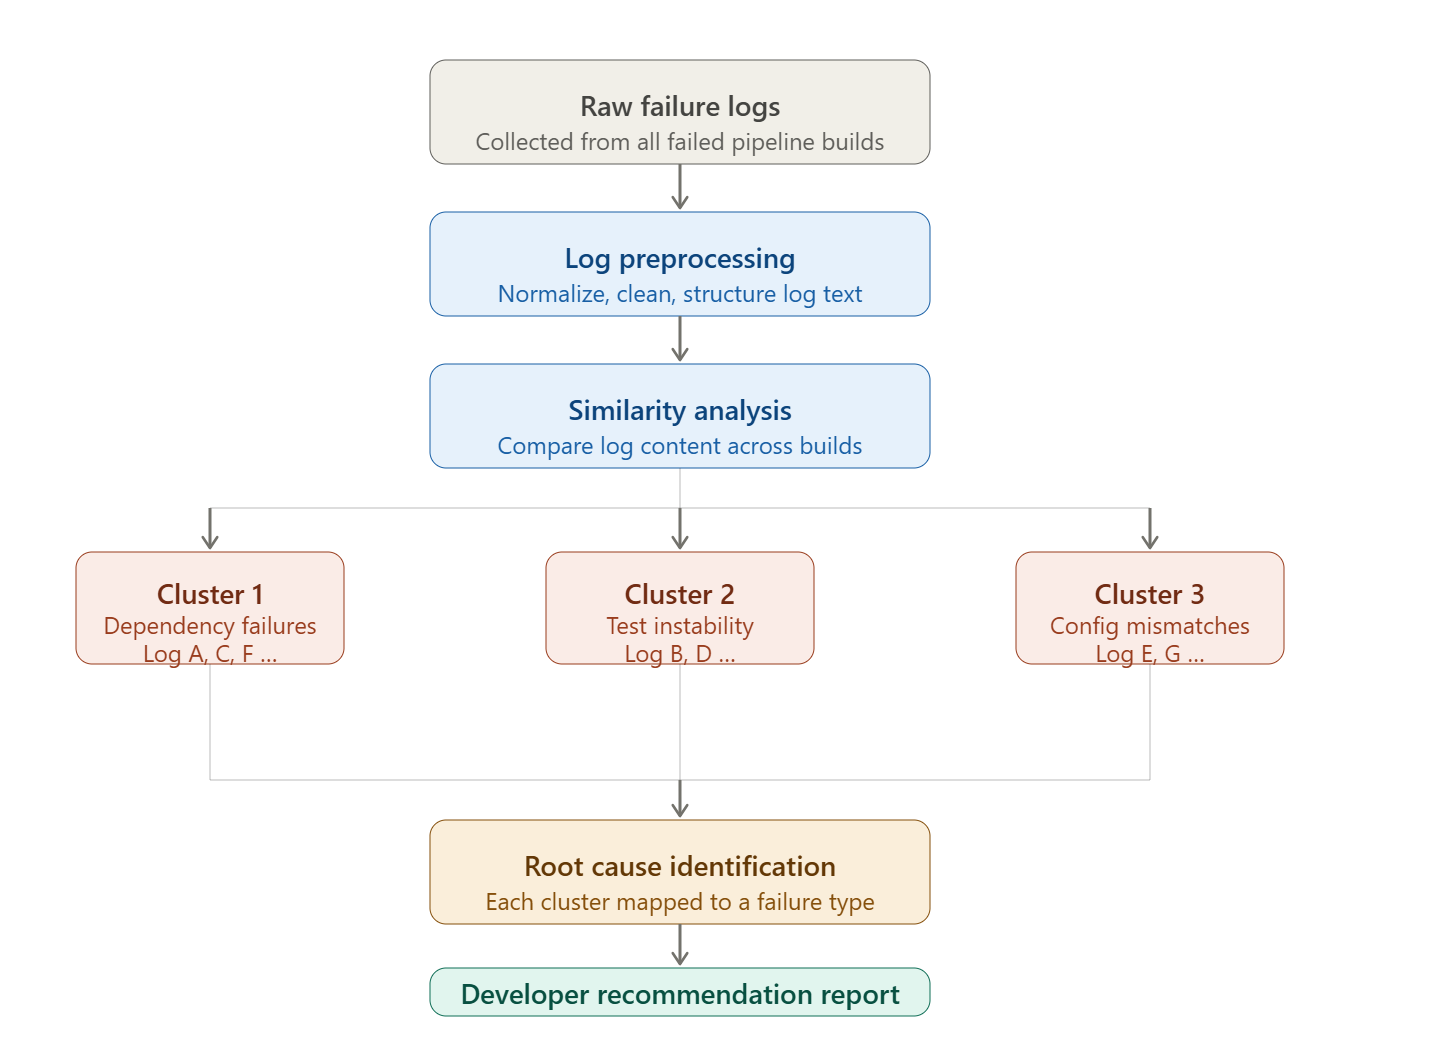
\includegraphics[width=0.78\textwidth]{fig_overview.png}
\caption{Log clustering flow for root cause analysis}
\label{fig:logflow}
\end{figure}

\minorhead{Feature Engineering}
Meaningful attributes are extracted from raw CI/CD data: code churn, files changed by type, failure rates of the repository and of the build's branch or pull request, the outcome of the previous build, builds still running, and commit timing. Every feature is checked against the availability registry, so nothing that is only known after a build finishes can be used (Section~\ref{sec:pipeline}).

\minorhead{Leakage-Safe Evaluation}
Models are evaluated with chronological walk-forward folds: they are trained only on the past and tested on the future. The metric is AUC measured within each repository, and confidence intervals come from bootstrapping over repositories~\cite{efron1993introduction}. External tests were pre-registered~\cite{nosek2018preregistration}: their plan was fixed and fingerprinted before any data was collected.
